\subsection{Caso d'uso UC5: Generazione del file PDF del progetto}
\begin{figure}[h] 
	\centering 
	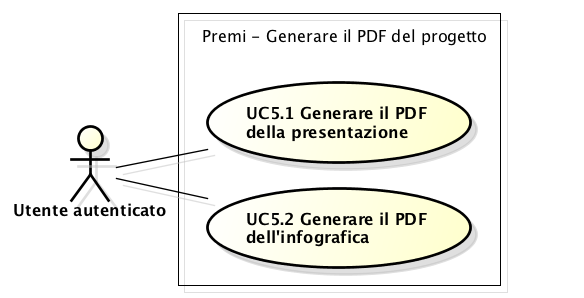
\includegraphics[scale=0.45] {img/UC5.png} 
	\caption{UC5 - Generazione PDF del progetto} 
\end{figure}

\begin{itemize}
	\item \textbf{Attori:} Utente autenticato, proprietario;
	\item \textbf{Scopo e descrizione:} L'utente ha aperto un progetto e vuole generare il PDF della presentazione o dell'infografica;
	\item \textbf{Precondizione:} L'utente ha un progetto aperto e il sistema è in attesa che selezioni la funzione di generazione del PDF;
	\item \textbf{Flusso principale degli eventi:}
	\begin{enumerate}
		\item L'utente seleziona la funzione di generazione del file PDF della presentazione [UC5.1];
		\item L'utente seleziona la funzione di generazione del file PDF dell'infografica [UC5.2].
	\end{enumerate}
	\item \textbf{Postcondizione:} Il sistema ha mandato in stampa la parte di progetto selezionata.
\end{itemize}

	\subsection{Caso d'uso UC5.1: Generare il PDF della presentazione}
	\begin{itemize}
		\item \textbf{Attori:} Utente autenticato, proprietario;
		\item \textbf{Scopo e descrizione:} L'utente ha aperto un progetto e vuole generare il PDF della presentazione;
		\item \textbf{Precondizione:} L'utente ha un progetto aperto e il sistema è in attesa che selezioni la funzione di generazione del PDF della presentazione;
		\item \textbf{Postcondizione:} Il sistema ha generato il PDF per l'utente e lo rende disponibile nel browser.
	\end{itemize}
	
	\subsection{Caso d'uso UC5.2: Generare il PDF dell'infografica}
	\begin{itemize}
		\item \textbf{Attori:} Utente autenticato, proprietario;
		\item \textbf{Scopo e descrizione:} L'utente ha aperto un progetto e vuole generare il PDF dell'infografica attraverso l'apposito comando;
		\item \textbf{Precondizione:} L'utente ha un progetto aperto di cui aveva creato l'infografica e il sistema è in attesa che selezioni la funzione di generazione del PDF dell'infografica;
		\item \textbf{Postcondizione:} Il sistema ha generato il PDF per l'utente e lo rende disponibile nel browser.
	\end{itemize}